\maketitle
\setcounter{page}{1}
\tableofcontents
\newpage
\pagenumbering{arabic}
\section{Theorie}
Der Photoeffekt beschreibt die Auslösung von Elektronen aus Metalloberflächen
durch das Einwirken von Licht. Dabei spielt die Natur des Lichtes eine Rolle.
Einige Phänomene, wie Beugung und Interferenz, lassen auf eine Wellennatur
des Lichtes schließen, während zum Beispiel der Compton-Effekt oder eben der
Photoeffekt nicht mit dem Wellenmodell zu vereinbaren sind. Um dieses Dilemma zu lösen,
wird die Quantenelektrodynamik genutzt. Diese enthält das Korpuskel- und Wellenmodell
als Grenzfälle. Bei einer großen Anzahl von Photonen lässt sich das Wellenmodell gut verwenden,
bei allen Wechselwirkungen von Licht mit Materie das Korpuskelmodell. \\
\\
In Abbildung \ref{fig:1} ist der schematische Aufbau zur Untersuchung des Photoeffekts abgebildet.
\begin{figure}[h]
  \centering
  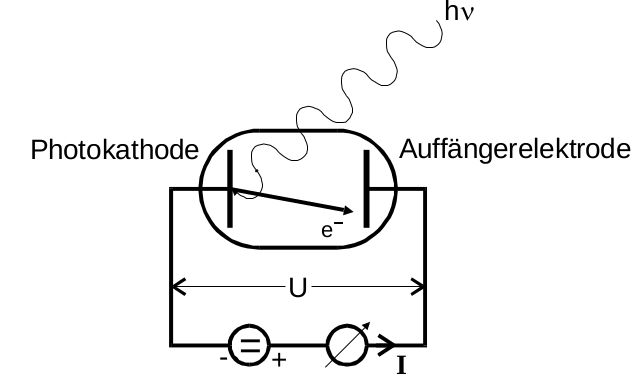
\includegraphics[scale=0.4]{aufbautheorie.png}
  \caption{Schema zur Untersuchung des Photoeffekts.}
  \label{fig:1}
\end{figure}
Dabei fällt monochromatisches Licht in einer Vakuumröhre auf eine als Photokathode bezeichnete Elektrode.
Ihr gegenüber liegt eine Elektrode, die ein positives Potential gegenüber der anderen Elektrode besitzt.
Diese nennt man Auffängerelektrode. Folgende Ergebnisse lassen sich aus diesem Aufbau gewinnen:
\begin{itemize}
  \item Es besteht ein proportionaler Zusammenhang zwischen der Zahl der pro Zeiteinheit ausgelösten
  Elektronen und der Lichtintensität.
  \item Die Energie der ausgelösten Elektronen ist proportional zur Frequenz des einfallenden
  Lichts, aber unabhängig von der Intensität.
  \item Es existiert eine Grenzfrequenz, unterhalb jener kein Photoeffekt auftritt.
\end{itemize}
All diese Erkenntnisse widersprechen der Wellennatur des Lichts, so müsste auch bei rotem
(sehr langwelligem) Licht nach genügend langer Einstrahlung ein Photoeffekt auftreten, d.h es
gäbe keine Grenzfrequenz. Weiterhin
wären die Energie der Photoelektronen, also die Elektronen, die mittels Photonenbeschuss aus dem Metall
gelöst wurden, abhängig von der Lichtintensität. Nimmt man stattdessen das Korpuskelmodell als gegeben an,
dann lassen sich alle experimentellen Resultate auf theoretischer Basis bestätigen. Im Einzelnen bedeutet dies:
\begin{itemize}
  \item Monochromatisches Licht mit der Frequenz $\nu$ besteht aus sich gradlinig bewegenden Photonen,
  die alle die Energie $E = h \nu$ besitzen.
  \item Beim Aufprall auf ein Elektron überrägt ein Photon eine Energie auf jenes Elektron. Diese spaltet
  sich nach
  \begin{equation}
    h \nu = A_k + E_{\symup{kin}}
    \label{eqn:1}
  \end{equation}
  auf. Dabei ist $A_k$ die Austrittsarbeit, die nötig ist, damit das Elektron den Potentialtopf
  des Metallgitters verlassen kann und $E_{\symup{kin}}$ die kinetische Energie des Elektrons
  nach dem Stoß. Mit \eqref{eqn:1} folgt, dass im Fall $h\nu < A_k$ kein Photoeffekt auftreten kann.
  Somit lässt sich das Auftreten einer Grenfrequenz erklären.
  \item Die Lichtintensität verhält sich proportional zur Zahl der Photonen pro Zeit- und Raumwinkeleinheit.
\end{itemize}

\section{Durchführung}
\subsection{Versuchsaufbau}
\begin{figure}[h]
  \centering
  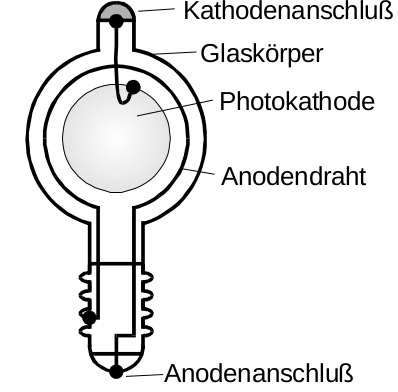
\includegraphics[scale=0.4]{aufbau.png}
  \caption{Schematischer Aufbau der Photozelle.}
  \label{fig:2}
\end{figure}
\subsection{Versuchsdurchführung}

\section{Auswertung}

\section{Diskussion}
\newpage
\nocite{*}
\printbibliography
